\section{Requirements}

\subsection{Functional requirements}

\begin{longtable}{|p{0.06\textwidth}|p{0.60\textwidth}|p{0.25\textwidth}|}
	\hline
	\textbf{ID} & \textbf{Requirement} & \textbf{Realised in} \\
	\hline
	\endhead
	F1 & Users can register with name, e-mail and password, log in and log out; a session lasts 7 days. & \texttt{routes/auth.\allowbreak{}ts}, \texttt{AuthPage} \\
	\hline
	F2 & Users can upload a match video (MP4, MOV, M4V, MKV, WebM, AVI, up to 1\,GB) with a title and an analysis mode and see the upload progress. & \texttt{routes/matches.\allowbreak{}ts}, \texttt{UploadPage} \\
	\hline
	F3 & Uploads are analysed asynchronously by workers through a job queue; the web request returns at once. & \texttt{queue.\allowbreak{}ts}, \texttt{worker.\allowbreak{}py} \\
	\hline
	F4 & The progress of each analysis (percentage and step) appears live, without reloading. & Socket.IO, \texttt{useMatchUpdates} \\
	\hline
	F5 & Players, goalkeepers, referees and the ball are detected and tracked. & \texttt{detector.\allowbreak{}py}, \texttt{tracker.\allowbreak{}py} \\
	\hline
	F6 & Positions are converted from image pixels to pitch coordinates in metres. & \texttt{homography.\allowbreak{}py} \\
	\hline
	F7 & People standing off the pitch and objects that only look like the ball are removed. & \texttt{cleanup.\allowbreak{}py} \\
	\hline
	F8 & Players are split into two teams; goalkeepers join their team; referees are recognised, also when the detector calls them players. & \texttt{clustering.\allowbreak{}py} \\
	\hline
	F9 & Each team's formation is recognised over time and every player gets a position label (LB, CB, ST\dots). & \texttt{clustering.\allowbreak{}py}, \texttt{positions.\allowbreak{}py} \\
	\hline
	F10 & Compactness, width, depth, distances, speeds and heatmaps are computed for teams, positions and the ball. & \texttt{metrics.\allowbreak{}py} \\
	\hline
	F11 & Results are drawn on the video (players, paths, team shape, ball, heatmaps), in sync frame by frame, also in full screen. & \texttt{VideoAnalysis}, \texttt{draw.\allowbreak{}ts} \\
	\hline
	F12 & A 2D tactical board shows the same moment from above with the current formations. & \texttt{drawBoard}, \texttt{VideoAnalysis} \\
	\hline
	F13 & Clicking a player shows the heatmap, path, distance, time visible and speeds of their position. & \texttt{PlayerPanel} \\
	\hline
	F14 & A language model writes a coaching report from the statistics; the report is stored. & \texttt{report.\allowbreak{}ts}, \texttt{CoachingReport} \\
	\hline
	F15 & Users can list, re-analyse, cancel and delete their own matches, and cannot reach other users' matches. & \texttt{routes/matches.\allowbreak{}ts} \\
	\hline
	F16 & Analysis can run on a remote GPU service, with automatic fallback to local analysis. & \texttt{remote.\allowbreak{}py}, \texttt{gpu\_\allowbreak{}server.\allowbreak{}py} \\
	\hline
	F17 & Videos of a full half (about 48 minutes, up to 1\,GB, any codec, 25 or 50\,fps) can be analysed. & \texttt{pipeline.\allowbreak{}py}, \texttt{remote.\allowbreak{}py} \\
	\hline
	\caption{Functional requirements}
	\label{tab:functional}
\end{longtable}

\subsection{Non-functional requirements}

\begin{table}[H]
	\centering
	\small
	\begin{tabular}{|p{0.06\textwidth}|p{0.18\textwidth}|p{0.67\textwidth}|}
		\hline
		\textbf{ID} & \textbf{Quality} & \textbf{Requirement} \\
		\hline
		N1 & Responsiveness & No web request waits for an analysis; heavy work runs in workers, and the dashboard stays usable meanwhile. \\
		\hline
		N2 & Scalability & Analysis capacity grows by adding workers or a GPU, without changes to the API or the dashboard. \\
		\hline
		N3 & Reliability & A failed or crashed analysis is retried; partial results are never shown; a lost GPU service falls back to local analysis; a job handed out twice is not analysed twice. \\
		\hline
		N4 & Security & Hashed passwords, script-proof session cookies, validated uploads, users isolated from each other, secrets kept out of the repository. \\
		\hline
		N5 & Deployability & One command starts the platform; every service has a container image, built and published automatically after the tests pass. \\
		\hline
		N6 & Maintainability & Typed code (TypeScript, Python type hints), validation of all external input, and automated unit, API and system tests on every change. \\
		\hline
		N7 & Usability & Overlays are synchronised to the exact video frame; the dashboard works in current browsers and adapts to smaller screens. \\
		\hline
		N8 & Efficiency & Long videos are streamed and never held in memory; the AI models are loaded once per worker process; memory stays below 5\,GB for a full half. \\
		\hline
	\end{tabular}
	\caption{Non-functional requirements}
	\label{tab:nonfunctional}
\end{table}

\subsection{Use cases}

\autoref{fig:usecase} shows the actors and their use cases. The registered user is the main actor. The AI worker is a system actor that drives the analysis and the progress updates, and the operator deploys and configures the platform outside the dashboard. \autoref{tab:stories} gives the main use cases as user stories.

\begin{figure}[H]
	\centering
	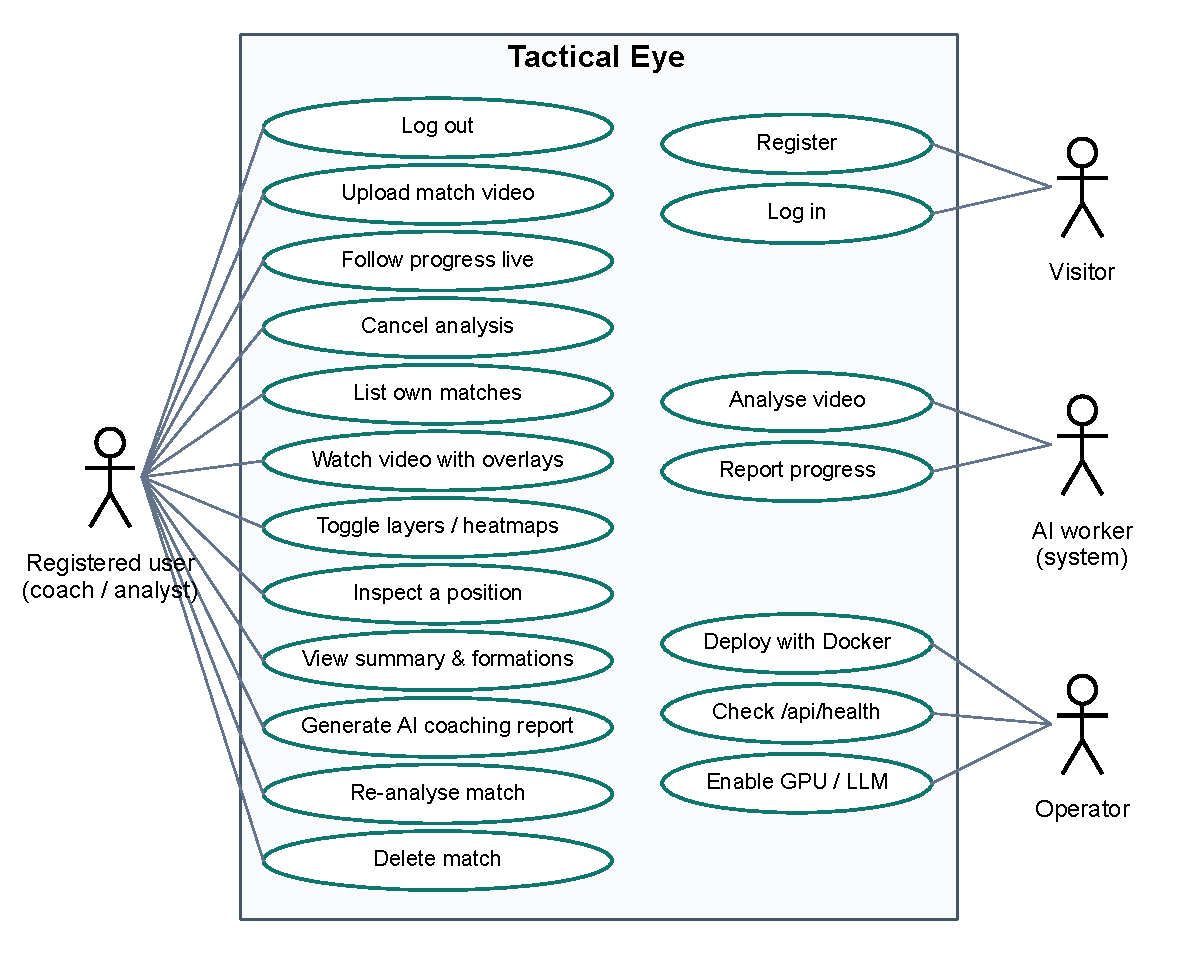
\includegraphics[width=\textwidth]{usecase}
	\caption{Use case diagram}
	\label{fig:usecase}
\end{figure}

\begin{longtable}{|p{0.18\textwidth}|p{0.74\textwidth}|}
	\hline
	\textbf{Use case} & \textbf{User story} \\
	\hline
	\endhead
	Upload a match & \emph{Given} a logged-in user with a video, \emph{when} they choose the file, a title and a mode and press \emph{Upload and analyse}, \emph{then} the video is stored, a queued match appears and its page opens. \\
	\hline
	Follow progress & \emph{Given} a match being analysed, \emph{when} the worker finishes a step, \emph{then} the progress bar and step label update on every open page of that user within a second. \\
	\hline
	Cancel & \emph{Given} a queued or running analysis, \emph{when} the user confirms \emph{Cancel analysis}, \emph{then} a queued job is removed at once and a running one stops within seconds, and the match shows as cancelled, or keeps its earlier results if it was a re-analysis. \\
	\hline
	Watch the analysis & \emph{Given} a finished match, \emph{when} the user plays the video, \emph{then} labels, paths and shapes stay on the players in every frame, also while the camera pans, and the board shows the same moment. \\
	\hline
	Inspect a position & \emph{Given} the analysis page, \emph{when} the user clicks a player, \emph{then} the player is highlighted and the heatmap, path, distance and speeds of their position are shown. \\
	\hline
	Generate a report & \emph{Given} a finished match and a configured model, \emph{when} the user presses \emph{Generate report}, \emph{then} a Markdown report based only on the statistics is shown and stored. \\
	\hline
	Retry after failure & \emph{Given} a worker that crashes during a job, \emph{when} its job lock expires, \emph{then} the job goes to a worker again; after a second failure the match is shown as failed with the reason. \\
	\hline
	\caption{User stories of the main use cases}
	\label{tab:stories}
\end{longtable}

\section{System architecture}

\subsection{Overview}

Tactical Eye is a distributed system with an asynchronous job queue (\autoref{fig:architecture}). It separates three parts with very different resource needs. The presentation tier is the React single-page application in the browser, which renders the dashboard and the overlays. The application tier is the Node.js API, which handles many short requests (log-in, uploads, lists, video streaming, live updates) and must stay responsive. The processing tier is the Python AI workers, which run long CPU- or GPU-bound analyses, one at a time.

\begin{figure}[H]
	\centering
	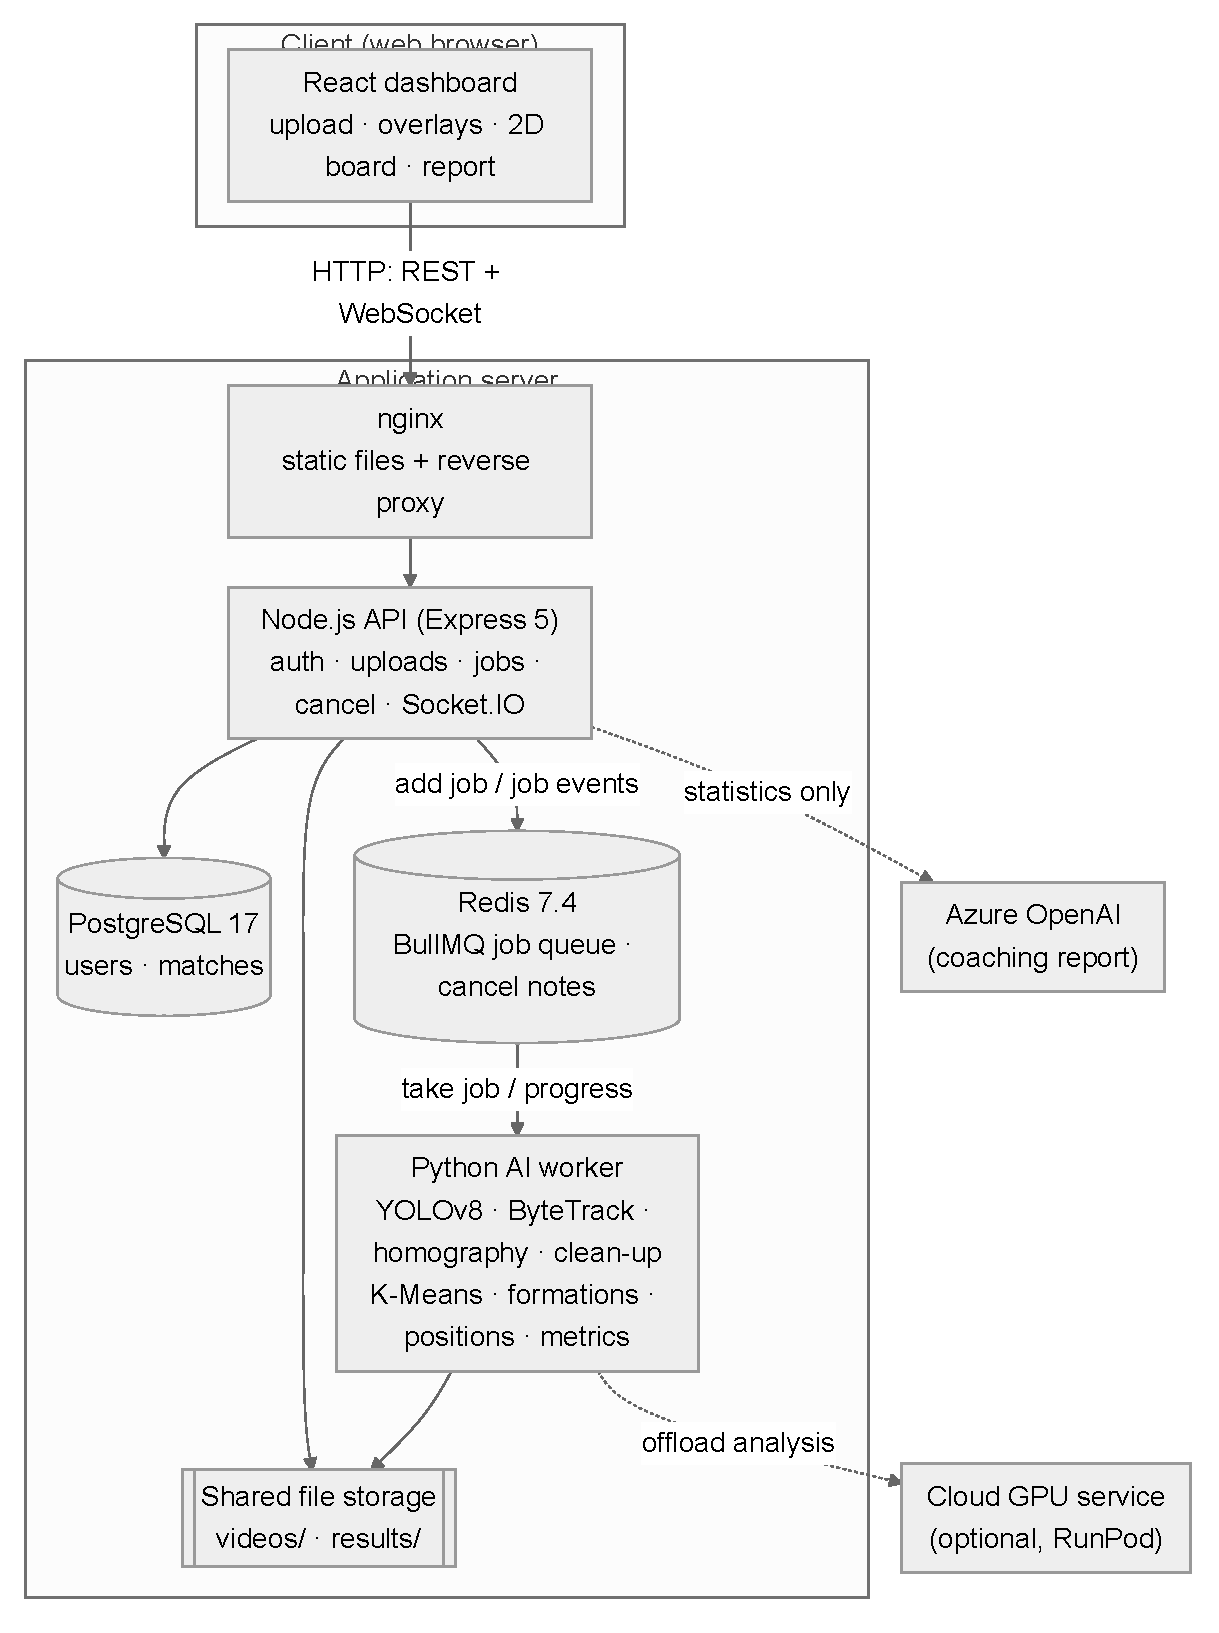
\includegraphics[width=0.8\textwidth]{architecture}
	\caption{Components and communication paths}
	\label{fig:architecture}
\end{figure}

The tiers talk through narrow interfaces: REST and a WebSocket between browser and API, a Redis-backed BullMQ queue~\cite{bullmq} between API and workers, a shared folder for videos and results, and the PostgreSQL database~\cite{postgres}, which only the API uses.

The central decision was that the API never runs an analysis itself. An upload creates a database row and a queue job and returns immediately, and workers pull jobs whenever they are free. I made this choice after the first prototype ran the pipeline inside the request handler: a 30-second clip kept the request open for 25 minutes, the browser gave up long before that, and a crash took the API down with it. With the queue, the API can serve many users while one worker spends an hour on a full half, workers can be added or removed without the API noticing, and jobs survive restarts because Redis stores them.

Progress flows the other way. The worker reports progress to the queue, the queue emits events, and the API, which listens to these events, updates the database and pushes the change to the browser over Socket.IO~\cite{socketio}. The browser never polls.

\subsection{Technology choices}

\autoref{tab:technologies} lists the technologies and their versions. The reasons behind the larger choices matter more than the list, so they follow the table.

\begin{longtable}{|p{0.13\textwidth}|p{0.33\textwidth}|p{0.45\textwidth}|}
	\hline
	\textbf{Layer} & \textbf{Technology} & \textbf{Purpose} \\
	\hline
	\endhead
	Frontend & React 19, TypeScript 6 & Component-based user interface~\cite{react}. \\
	\cline{2-3}
	& Vite 8, Vitest 4 & Development server, production bundler and unit tests~\cite{vite,vitest}. \\
	\cline{2-3}
	& React Router 8, Tailwind CSS 4 & Client-side routing; utility-first styling~\cite{tailwind}. \\
	\cline{2-3}
	& Socket.IO client 4.8, react-markdown 10 & Live updates; rendering the coaching report. \\
	\cline{2-3}
	& HTML5 Canvas, \texttt{request\allowbreak{}Video\allowbreak{}Frame\allowbreak{}Callback}, Fullscreen API & Frame-synchronised drawing and full-screen view~\cite{rvfc}. \\
	\hline
	Backend & Node.js 24, Express 5, TypeScript 6 & REST API~\cite{express}; Express 5 passes errors of async handlers to the error middleware. \\
	\cline{2-3}
	& Prisma 7, PostgreSQL 17 & Typed database access and migrations~\cite{prisma,postgres}. \\
	\cline{2-3}
	& BullMQ 6, Redis 7.4 & Job queue, queue events and the cancel notes~\cite{bullmq,redis}. \\
	\cline{2-3}
	& Socket.IO 4.8, Zod 4 & WebSocket server; validation of requests and settings. \\
	\cline{2-3}
	& Multer 2, bcryptjs 3, jsonwebtoken 9 & Uploads, password hashing, session tokens~\cite{jwt}. \\
	\cline{2-3}
	& openai 6 (\texttt{AzureOpenAI} client) & Coaching reports~\cite{azureopenai}. \\
	\cline{2-3}
	& Vitest 4, SuperTest 7 & API tests against a real test database~\cite{vitest,supertest}. \\
	\hline
	AI worker & Python 3.12 & Worker language. \\
	\cline{2-3}
	& Ultralytics 8.4 (YOLOv8), PyTorch 2.14 & Object and keypoint detection~\cite{yolov8,pytorch}. \\
	\cline{2-3}
	& trackers 2.6 (ByteTrack), supervision 0.31 & Multi-object tracking and detection utilities~\cite{bytetrack,supervision}. \\
	\cline{2-3}
	& OpenCV 5, NumPy 2.5, pandas 3, SciPy 1.18, scikit-learn 1.9 & Homography, colour spaces, data processing, Hungarian algorithm, convex hulls, K-Means~\cite{opencv,sklearn}. \\
	\cline{2-3}
	& PyAV 19 (libx264, dav1d) & Reading any codec, writing the H.264 playback copy~\cite{pyav}. \\
	\cline{2-3}
	& bullmq 3.4 (Python), redis 8, psutil & Queue consumer compatible with Node.js BullMQ; cancel notes; memory measurement. \\
	\cline{2-3}
	& FastAPI, uvicorn, httpx, pytest & Remote GPU service and its client; unit tests~\cite{pytest}. \\
	\hline
	Operations & Docker, Docker Compose, nginx 1.27 & Containers, orchestration, reverse proxy~\cite{docker}. \\
	\cline{2-3}
	& GitHub Actions, GitHub Container Registry & CI/CD pipeline and image registry~\cite{ghactions}. \\
	\cline{2-3}
	& Azure OpenAI (\texttt{gpt-5-mini}), RunPod (NVIDIA L4) & External language model and GPU~\cite{runpod}. \\
	\hline
	\caption{Technologies and versions}
	\label{tab:technologies}
\end{longtable}

TypeScript runs on both the frontend and the API, so the shapes of shared data (a match, the results file) are written once and checked by the compiler on both sides. The worker is in Python because the computer vision ecosystem is: PyTorch, Ultralytics, OpenCV and pandas have no comparable counterparts in Node.js. Two languages need a queue that both understand. Celery would have tied the queue to Python and RabbitMQ would have added another server; BullMQ has a Node.js and a Python implementation that share the same Redis data structures, so the API adds jobs in TypeScript and the worker takes them in Python.

PostgreSQL won over MongoDB because the data is relational (users own matches, and every query filters by owner) and because its JSON column still lets me store the loosely structured match summary without a schema for every number. I chose Prisma over writing SQL by hand because it generates a typed client and a migration file for every schema change; the \texttt{CANCELLED} status, for example, became a one-line schema change and a generated \texttt{ALTER TYPE} migration.

For detection I used YOLOv8 with weights that Roboflow trained on broadcast football~\cite{roboflowsports}. Training my own model was not realistic: it needs thousands of annotated frames and GPU time I did not have, while these weights already know the classes ball, goalkeeper, player and referee. ByteTrack~\cite{bytetrack} was chosen because it keeps low-confidence detections in a second matching round, which is exactly what happens to partly hidden players in crowded penalty areas.

Drawing the analysis in the browser instead of burning it into a new video was a deliberate choice as well. A rendered video would have been simpler to show, but every layer combination would need its own video, nothing could be clicked, and a full half would mean rendering another gigabyte. Drawing on a canvas from the results file lets the user switch layers, select players and step through frames, at the cost of the synchronisation work described in \autoref{sec:overlay-sync}.

\subsection{Layers inside the services}

Each service is layered as well. In the frontend, pages (one per route) compose reusable components; all server communication goes through one API module (\texttt{api.\allowbreak{}ts}) and one WebSocket hook (\texttt{useMatchUpdates}); and the pure analysis modules (\texttt{timeline.\allowbreak{}ts}, \texttt{geometry.\allowbreak{}ts}, \texttt{draw.\allowbreak{}ts}) contain the overlay logic with no dependency on React, which also makes them easy to unit-test. In the backend, routes handle HTTP and validate input, then call service modules (\texttt{queue.\allowbreak{}ts}, \texttt{storage.\allowbreak{}ts}, \texttt{report.\allowbreak{}ts}, \texttt{colours.\allowbreak{}ts}, \texttt{auth.\allowbreak{}ts}), which use the Prisma client in \texttt{db.\allowbreak{}ts}. \texttt{config.\allowbreak{}ts} validates all settings at start-up. In the worker, the queue adapter (\texttt{worker.\allowbreak{}py}) knows nothing about computer vision; it calls the pipeline orchestrator (\texttt{pipeline.\allowbreak{}py}), which chains independent stage modules that exchange pandas DataFrames.

\subsection{End-to-end flow}

\autoref{fig:sequence} and \autoref{fig:sequence-progress} follow one upload through the system. The upload is checked and stored, a job is queued, and the worker takes it (\autoref{fig:sequence}); the worker then reports progress that the API relays to the browser, and on completion the browser downloads the results and the playback video (\autoref{fig:sequence-progress}).

\begin{landscape}
	\begin{figure}
		\centering
		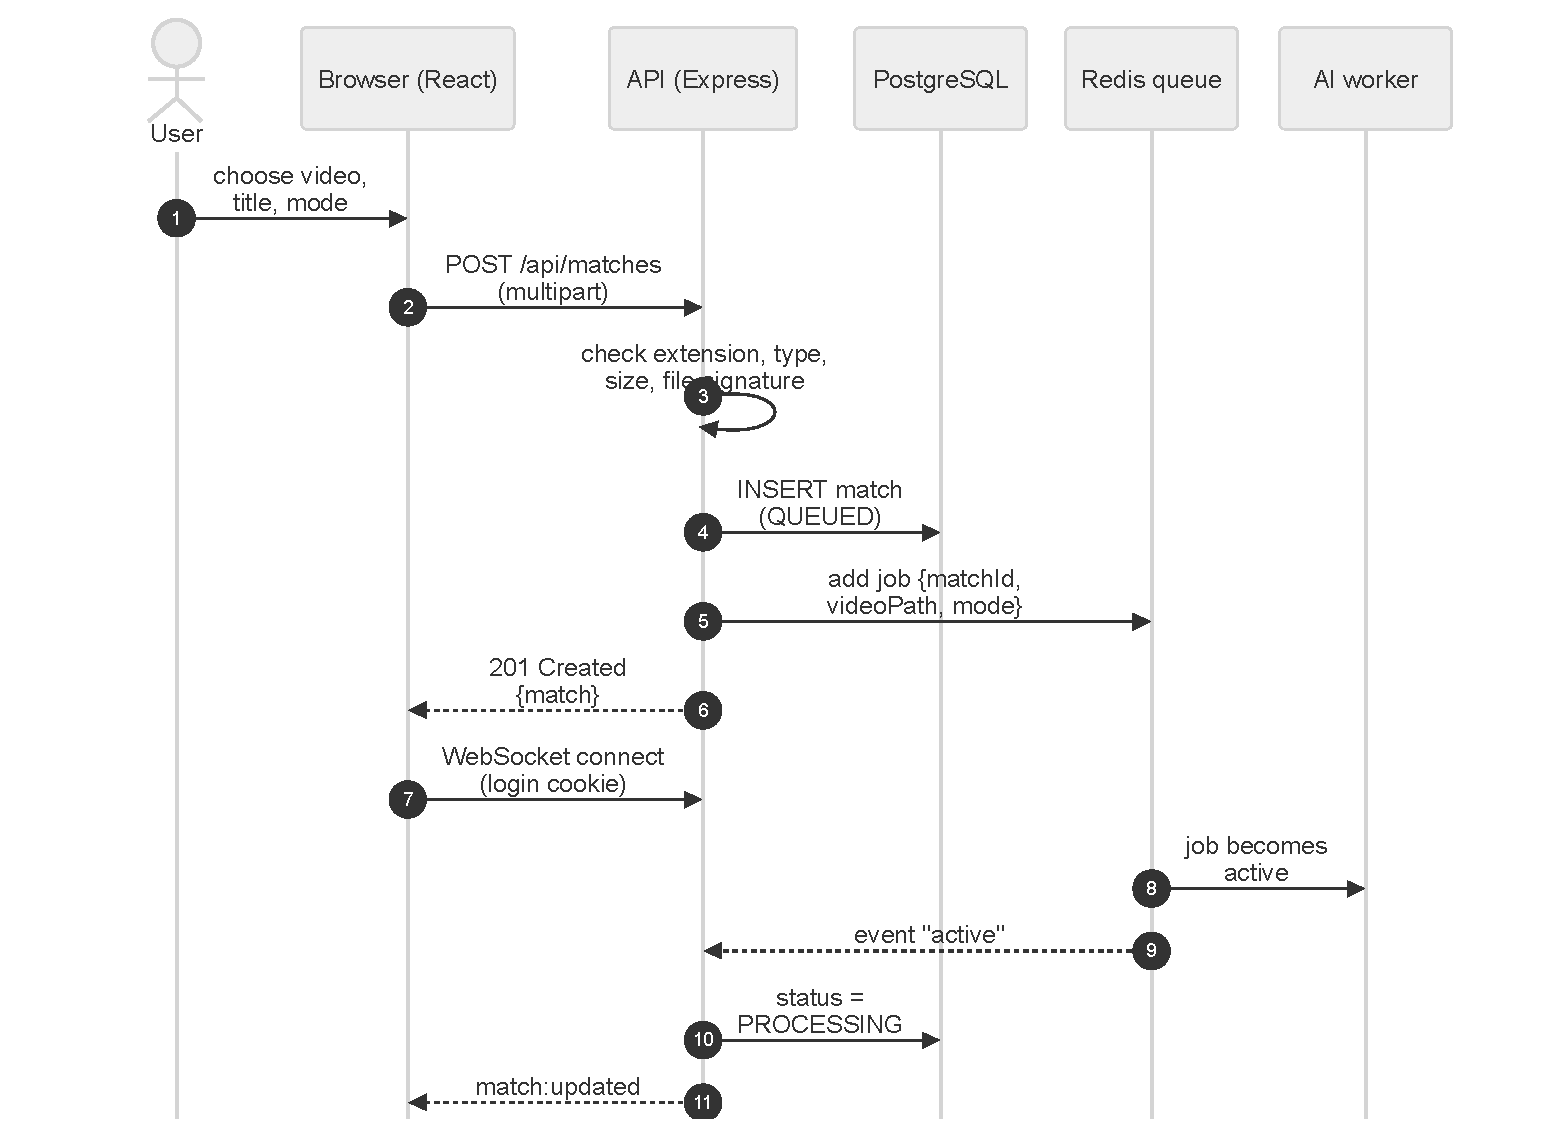
\includegraphics[width=\linewidth,height=0.86\textheight,keepaspectratio]{sequence_upload}
		\caption{Sequence of an upload, part 1: storing the video and queueing the job}
		\label{fig:sequence}
	\end{figure}
\end{landscape}

\begin{landscape}
	\begin{figure}
		\centering
		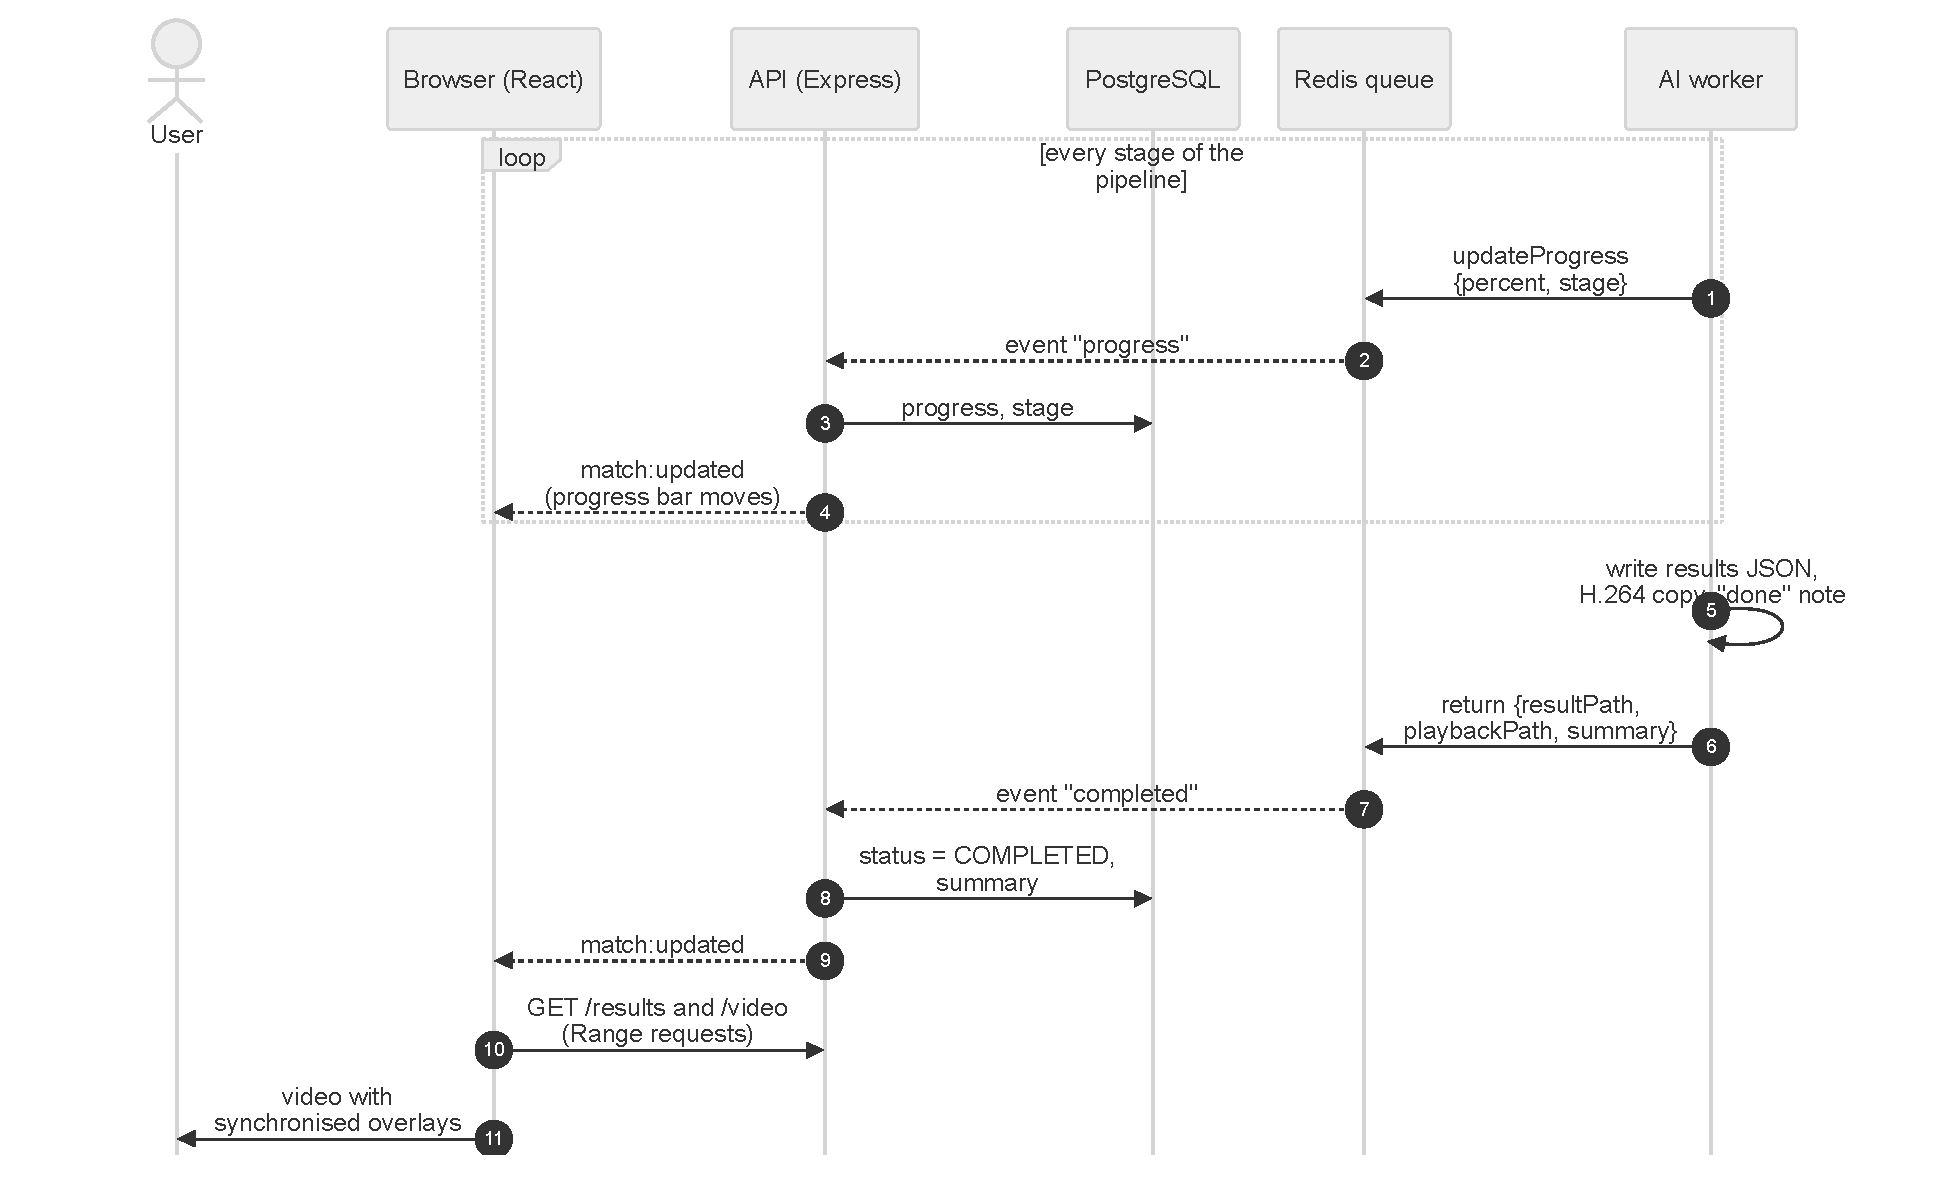
\includegraphics[width=\linewidth,height=0.86\textheight,keepaspectratio]{sequence_progress}
		\caption{Sequence of an upload, part 2: live progress, completion and playback}
		\label{fig:sequence-progress}
	\end{figure}
\end{landscape}

\section{Deployment and CI/CD}

\subsection{Containers}

Every service has its own \texttt{Dockerfile}, and \texttt{docker-compose.\allowbreak{}yml} describes how they work together (\autoref{fig:deployment}). The file uses a Compose profile: \texttt{docker compose up -d} starts only PostgreSQL and Redis, which suits development, when the three application services run directly on the developer's machine with hot reloading, while \texttt{docker compose --profile app up -d --build} starts the whole platform.

\begin{landscape}
	\begin{figure}
		\centering
		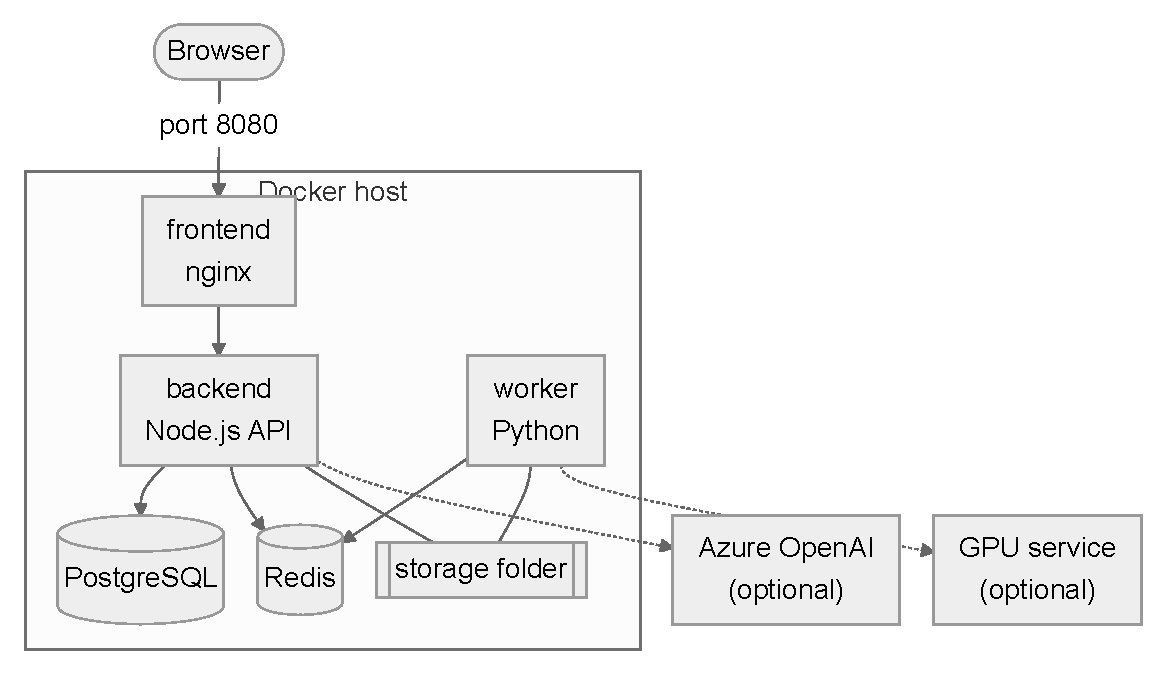
\includegraphics[width=\linewidth,height=0.86\textheight,keepaspectratio]{deployment}
		\caption{Deployment diagram}
		\label{fig:deployment}
	\end{figure}
\end{landscape}

\begin{table}[H]
	\centering
	\small
	\begin{tabular}{|p{0.11\textwidth}|p{0.22\textwidth}|p{0.58\textwidth}|}
		\hline
		\textbf{Service} & \textbf{Base image} & \textbf{Build and start-up} \\
		\hline
		frontend & \texttt{node:24-alpine} $\rightarrow$ \texttt{nginx:1.27-alpine} & Multi-stage build: the first stage runs \texttt{npm ci} and \texttt{npm run build}; only the static output is copied into the small nginx image. \\
		\hline
		backend & \texttt{node:24-alpine} & \texttt{npm ci} and \texttt{prisma generate}; on start, \texttt{prisma migrate deploy} applies pending migrations, then the API starts. Health check on \texttt{/api/health}. \\
		\hline
		worker & \texttt{python:3.12-slim} & OpenCV's system libraries, the CPU build of PyTorch and the pinned requirements. The models are mounted read-only from \texttt{worker/models}, so the image (about 3.4\,GB) contains no model files. \\
		\hline
		postgres & \texttt{postgres:17-alpine} & Data in a named volume; health check with \texttt{pg\_\allowbreak{}isready}. \\
		\hline
		redis & \texttt{redis:7.4-alpine} & Append-only file enabled, so queued jobs survive a Redis restart; health check with \texttt{redis-cli ping}. \\
		\hline
	\end{tabular}
	\caption{Container images}
	\label{tab:images}
\end{table}

The backend and worker containers mount the same \texttt{./storage} folder at \texttt{/storage}. The database stores only relative paths such as \texttt{videos/3f2a\dots.\allowbreak{}mp4}, and each service joins them with its own \texttt{STORAGE\_\allowbreak{}DIR}, so both agree on the files although they see the folder at different absolute paths.

\subsection{Reverse proxy}

In the container deployment the browser only talks to nginx on port 8080. nginx serves the built dashboard and forwards \texttt{/api/} and \texttt{/socket.\allowbreak{}io/} to the backend (\autoref{code:nginx}). Because everything comes from one origin, the log-in cookie and the WebSocket need no cross-origin configuration. Uploads are streamed straight through (\texttt{proxy\_\allowbreak{}request\_\allowbreak{}buffering off}), and the body limit matches the API's 1\,GB limit. Unknown paths such as \texttt{/matches/abc} return \texttt{index.\allowbreak{}html}, so deep links into the single-page application work.

\begin{lstlisting}[style=plain, caption={nginx configuration (excerpt from \texttt{frontend/nginx.\allowbreak{}conf})}, label={code:nginx}]
client_max_body_size 1050m;   # the API's 1 GB limit plus form overhead

location /api/ {
    proxy_pass http://backend:4000;
    proxy_request_buffering off;  # stream uploads straight to the API
    proxy_read_timeout 300s;
}
location /socket.io/ {
    proxy_pass http://backend:4000;
    proxy_http_version 1.1;
    proxy_set_header Upgrade $http_upgrade;  # WebSocket handshake
    proxy_set_header Connection "upgrade";
}
location / {
    try_files $uri $uri/ /index.html;       # single-page app fallback
}
\end{lstlisting}

\subsection{Continuous integration and delivery}
\label{sec:cicd}

The GitHub Actions workflow \texttt{.\allowbreak{}github/workflows/ci.\allowbreak{}yml} runs on every push and pull request (\autoref{fig:cicd}). Three jobs run in parallel. The backend job starts PostgreSQL and Redis as service containers, type-checks the API and runs its 42 Vitest and SuperTest tests against a real test database. The frontend job lints the code with oxlint, runs the 23 unit tests of the overlay mathematics and builds the production bundle, which includes the TypeScript check. The worker job installs the CPU build of PyTorch and runs the 43 pytest tests.

When all three pass, the system job downloads the two AI models (cached between runs), starts the whole platform with Docker Compose and runs the 11 system tests against it from the outside, including a real analysis of a 3-second clip and the cancelling of a running analysis. Only then does the images job build the three Docker images; on pushes to \texttt{main} it also publishes them to the GitHub Container Registry, tagged \texttt{latest} and with the commit hash. Every published image has therefore passed every test level, and any earlier version can be redeployed. \autoref{ch:testing} describes the tests themselves.

\begin{figure}[H]
	\centering
	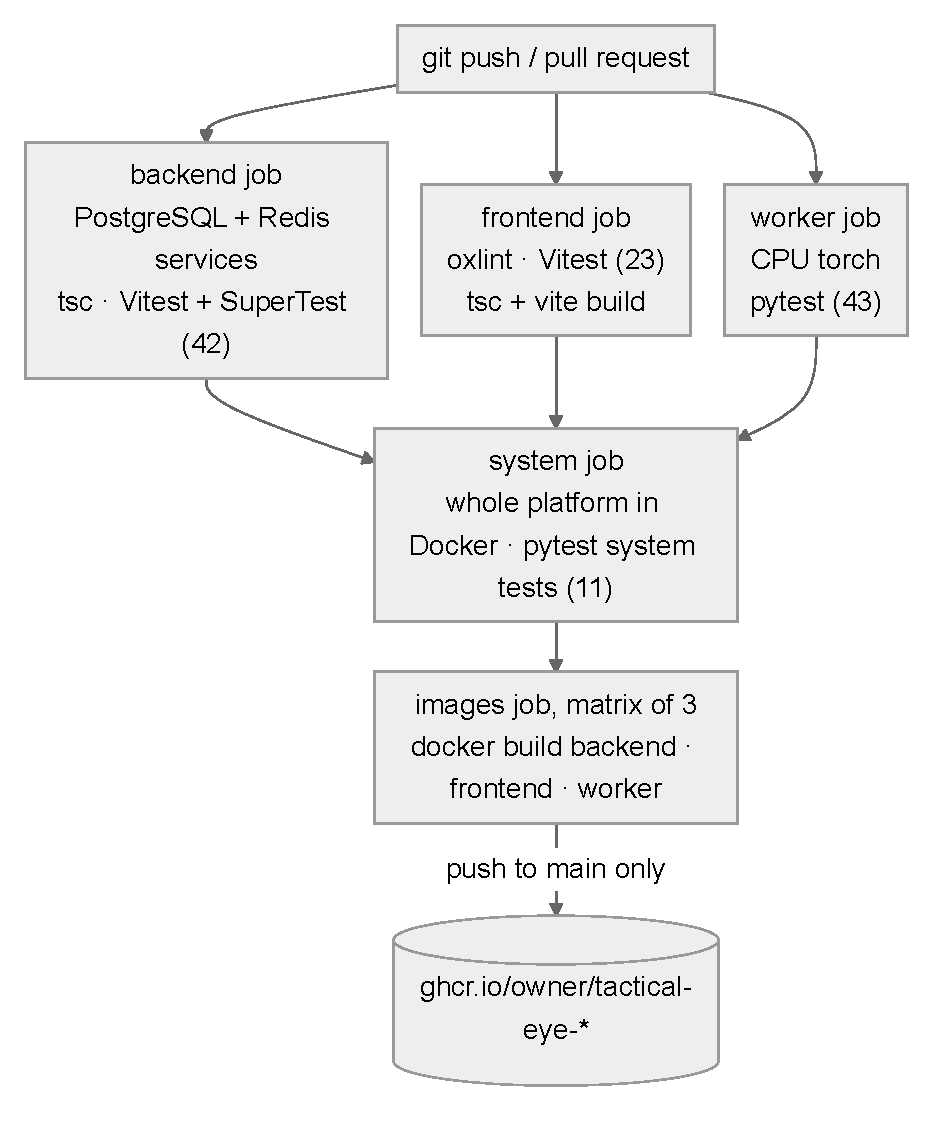
\includegraphics[width=0.7\textwidth]{cicd}
	\caption{The CI/CD pipeline}
	\label{fig:cicd}
\end{figure}

\subsection{Configuration}

All settings come from environment variables (\autoref{tab:env}). Locally they are read from the \texttt{.\allowbreak{}env} file in the repository root; in Docker, Compose passes them to the containers. The API checks its configuration with a Zod schema at start-up (\autoref{code:config}), so a missing or malformed value stops the server at once with a clear message instead of failing later inside a request. Secrets exist only in \texttt{.\allowbreak{}env}, which version control ignores.

\begin{lstlisting}[language=TypeScript, caption={Validated configuration (excerpt from \texttt{backend/src/config.\allowbreak{}ts})}, label={code:config}]
const EnvSchema = z.object({
  DATABASE_URL: z.string().min(1),
  REDIS_URL: z.string().default("redis://localhost:6379"),
  JWT_SECRET: z.string().min(32, "JWT_SECRET must be at least 32 characters"),
  // 1 GB: enough for a full half of a match (about 45 minutes).
  MAX_UPLOAD_MB: z.coerce.number().positive().default(1024),
  COOKIE_SECURE: z.enum(["true", "false"]).optional(),
});
const parsed = EnvSchema.safeParse(process.env);
if (!parsed.success) {
  console.error("Invalid configuration:\n" + z.prettifyError(parsed.error));
  process.exit(1);
}
\end{lstlisting}
